\chapter{Design and Architecture} \label{ch:architecture}

\section{Overview}\label{sec:overview}

The Prometheus Kotlin client library is architected to provide a comprehensive, \ac{KMP} solution for
defining, collecting, and exporting application metrics in a manner compliant with the Prometheus monitoring ecosystem.
Its design supports all core Prometheus metric types—namely, counters, gauges, histograms, and summaries—enabling
accurate instrumentation of application behavior and performance across diverse runtime environments such as \ac{JVM} and native platforms.

\begin{figure}[H]
    \centering
    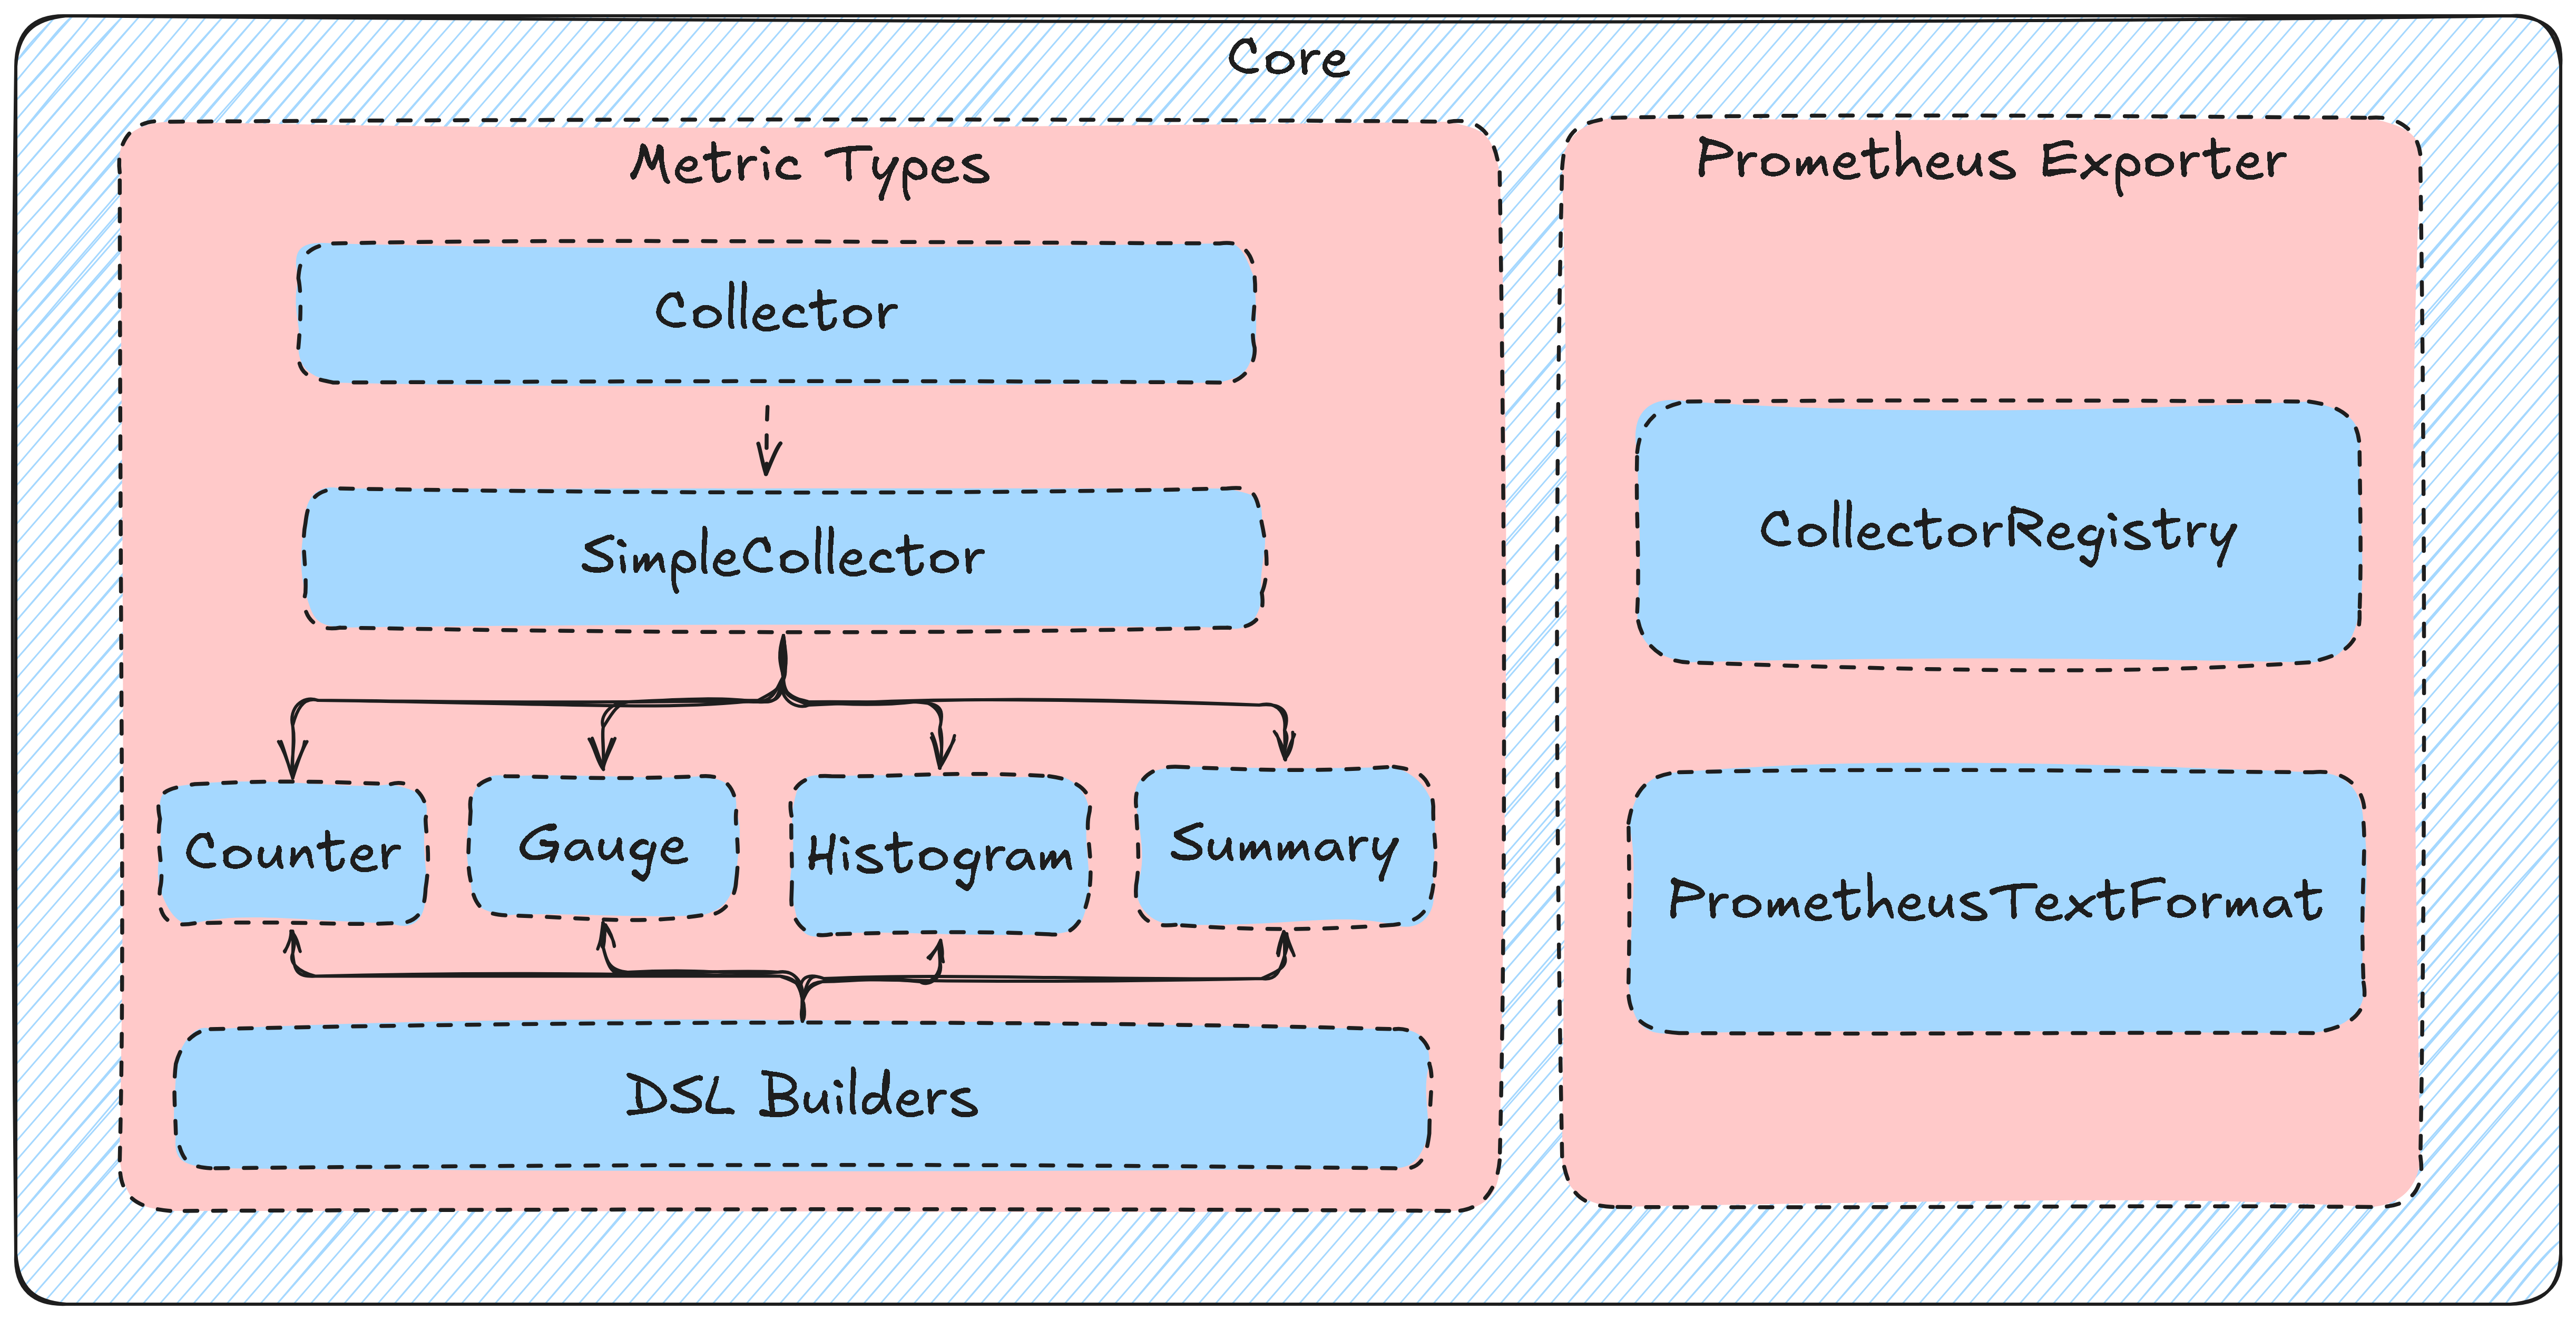
\includegraphics[width=\linewidth, keepaspectratio]{./figures/core_arch}
    \caption{Core Architecture}
\end{figure}

Central to the architecture is the \texttt{CollectorRegistry}, a thread-safe, platform-agnostic component responsible for managing metric collectors and aggregating their samples.
This registry acts as the single source of truth for all registered metrics and ensures that metric collection can occur concurrently without data races or inconsistencies.

The metric model is structured around an extensible hierarchy of collector abstractions.
The abstract base class \texttt{Collector} defines the core contract for metric collectors, while the \texttt{SimpleCollector} subclass handles metrics with label support by managing child metric instances identified by unique label sets.
Concrete implementations such as \texttt{Counter}, \texttt{Gauge}, \texttt{Histogram}, and \texttt{Summary} extend this hierarchy, encapsulating their specific semantics and data aggregation strategies.

For data exposure, the library includes an exporter module that serializes collected metrics into the Prometheus
text-based exposition format (version 0.0.4)\cite{prometheus_exposition_formats}.
This serialization strictly adheres to the Prometheus scraping protocol, ensuring compatibility with Prometheus servers and related tooling.
To preserve the multiplatform nature of the core library, the HTTP server components responsible for exposing
metrics over the network are isolated into a separate \ac{JVM}-specific module utilizing the Ktor framework.
This modularization prevents platform-specific dependencies from polluting the core library and allows users to selectively include HTTP exposition features as needed.

In summary, the architecture is characterized by:

\begin{itemize}
    \item \textbf{Portability}: Core metric collection logic is platform-independent and compatible with all Kotlin targets.
    \item \textbf{Modularity}: Separation of core logic and platform-specific integrations promotes maintainability and extensibility.
    \item \textbf{Thread Safety}: Use of multiplatform concurrency primitives ensures safe concurrent access to metrics.
    \item \textbf{Standards Compliance}: Exported metrics conform to Prometheus exposition format, guaranteeing interoperability.
\end{itemize}

This architecture provides a scalable and robust foundation for implementing reliable metric instrumentation in Kotlin applications, empowering developers to integrate with Prometheus-based monitoring pipelines effortlessly.

\subsection{Intended Usage and Integration Scenarios}\label{subsec:intended-usage-and-integration-scenarios}

This library is designed to provide a lightweight, idiomatic Prometheus client implementation for Kotlin
applications, with full support for \ac{KMP}.
It exposes a core \ac{API} for defining, updating, and exporting Prometheus metrics without relying on any platform-specific construct.

The architecture is modular, enabling developers to use only what they need.
This allows the library to be integrated into a wide range of
applications, such as:

\begin{itemize}
    \item \textbf{Kotlin Multiplatform background services}, including command-line tools or daemon-like processes, where metrics can be logged or periodically collected by another component.
    \item \textbf{Kotlin/JVM web applications}, which can expose metrics over HTTP by including an additional module that integrates with a web framework (e.g., Ktor).
\end{itemize}

The library aims to support both simple and advanced scenarios.
For example, developers writing a \ac{JVM}-based backend in Ktor can add the HTTP exposition module to expose
metrics at a \texttt{/metrics} endpoint.
Conversely, developers building a multiplatform application that collects metrics locally can use only the core module, avoiding unnecessary dependencies.

This flexibility ensures that the library remains lightweight, portable, and easy to integrate into various environments.


\section{Module Structure}\label{sec:module-structure}

\begin{figure}[H]
    \centering
    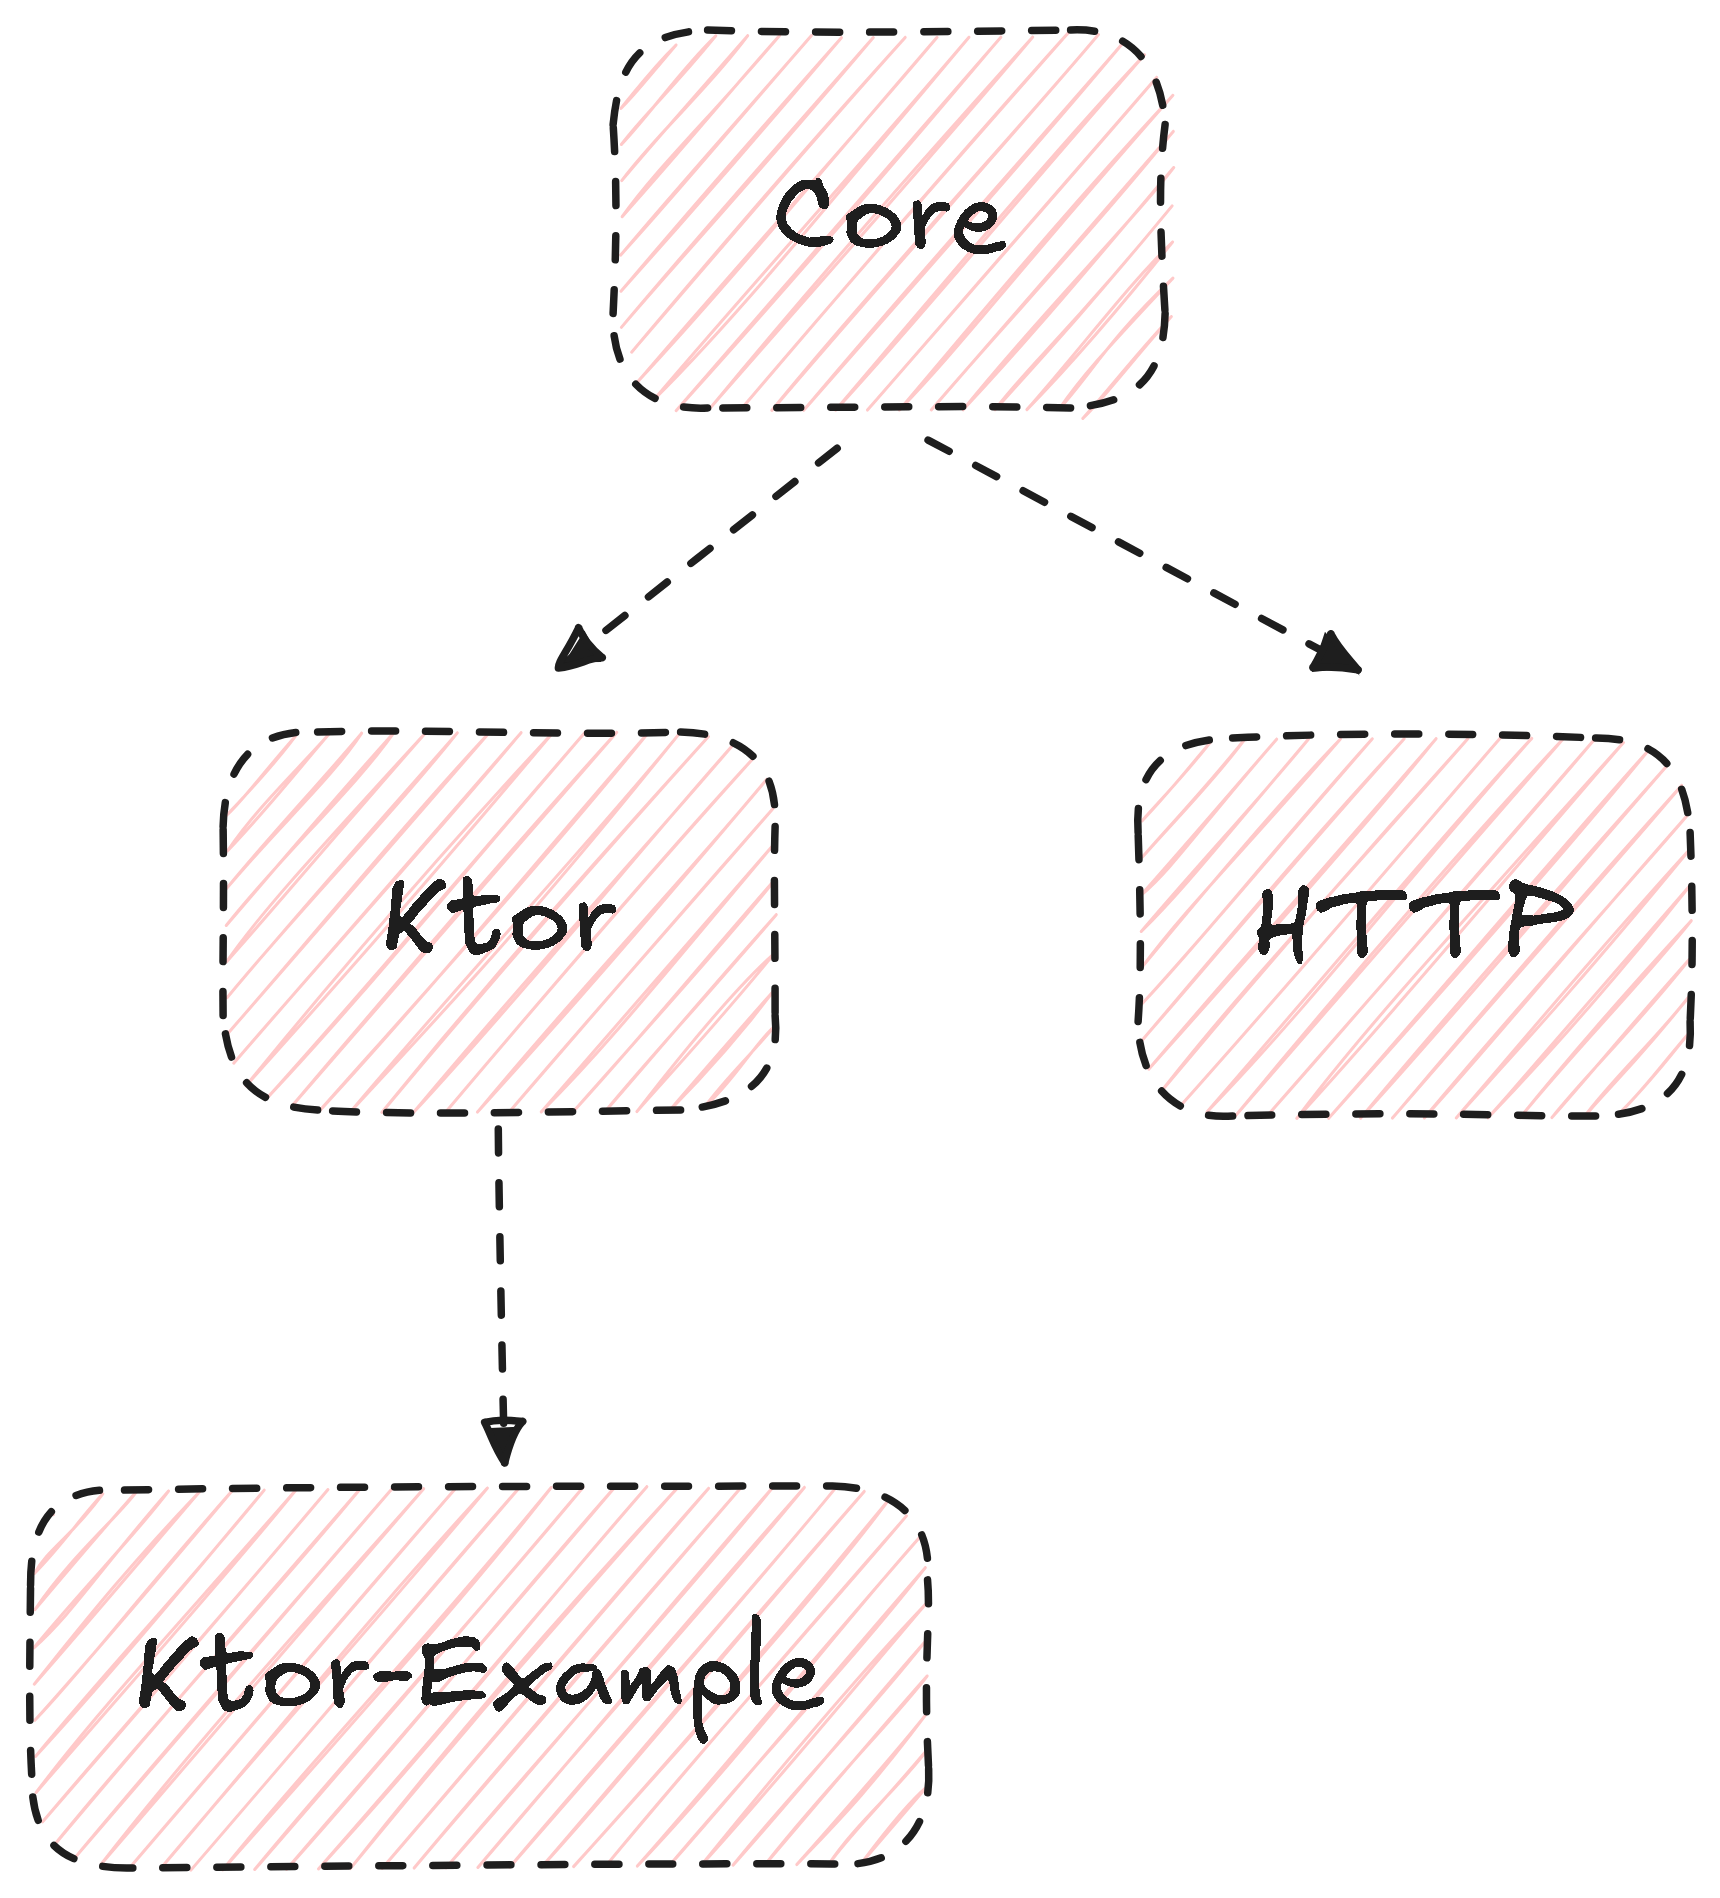
\includegraphics[width=0.75\linewidth, keepaspectratio]{./figures/module_dependencies}
    \caption{Module Dependencies}
\end{figure}

The Prometheus client library is organized into a modular architecture to ensure clean separation of concerns, platform flexibility, and ease of use across different application environments.
Each module encapsulates a specific layer of functionality, ranging from the core metric definitions to optional platform-specific integrations for HTTP exposition.
The current structure consists of the following modules:


\begin{itemize}
    \item \textbf{core} --- A \ac{KMP} module containing the core logic of the Prometheus client library.
    It includes the metric types (e.g., \texttt{Counter}, \texttt{Gauge}), the registry mechanism, the text
    exposition formatter, and the \ac{DSL} for defining metrics.
    This is the only module that is \ac{KMP}-compatible and targets multiple platforms.

    \item \textbf{ktor} --- A \ac{JVM}-only module that integrates the core library with the Ktor web framework.
    It provides a route handler that exposes the registered metrics via an HTTP endpoint (typically at \texttt{/metrics}). Additionally, it automatically registers useful server-side metrics such as request counts, durations, and response statuses, giving developers immediate visibility into their application's performance.

    \item \textbf{http} --- A lightweight \ac{JVM}-only module that provides a minimal HTTP server for metrics
    exposition, independent of any web framework.
    It is specifically designed for users who want to expose metrics in environments that either lack an HTTP server or rely on unsupported frameworks.
    This makes it ideal for background workers, command-line tools, or embedded applications where adopting a full web stack would be excessive.

    \item \textbf{ktor-example} --- A self-contained demonstration module showing how to integrate the library in a real Ktor web application.
    This module is fully Dockerized and includes a complete monitoring stack, featuring Prometheus and Grafana containers for out-of-the-box metrics visualization.
    Additionally, it contains load simulation logic that periodically generates synthetic requests, allowing users to observe dynamic metric changes in real time.

    \item \textbf{ktor-example/docker-compose.yml} --- Provides the configuration to spin up the example service alongside Prometheus and Grafana.
    The Prometheus configuration is preloaded to scrape the Ktor application, and Grafana dashboards are preconfigured to visualize common metrics.
\end{itemize}

This modular design ensures that users only depend on the components they need.
For example, a \ac{KMP} application targeting native platforms can rely solely on \texttt{core}, while a JVM backend
can optionally include \texttt{ktor} or \texttt{http} depending on its architectural requirements.
The \texttt{ktor-example} module provides a practical blueprint for integration but is not intended to be used as a dependency.


\section{Metric Model}\label{sec:metric-model}

The metric model of the Prometheus Kotlin client library provides abstractions for the four fundamental Prometheus metric types: \texttt{Counter}, \texttt{Gauge}, \texttt{Histogram}, and \texttt{Summary}. Each type has its specific semantics and API designed to facilitate common monitoring tasks in an idiomatic Kotlin manner.

\subsection{Metric Types Overview}\label{subsec:metric-types-overview}

\begin{figure}[H]
    \centering
    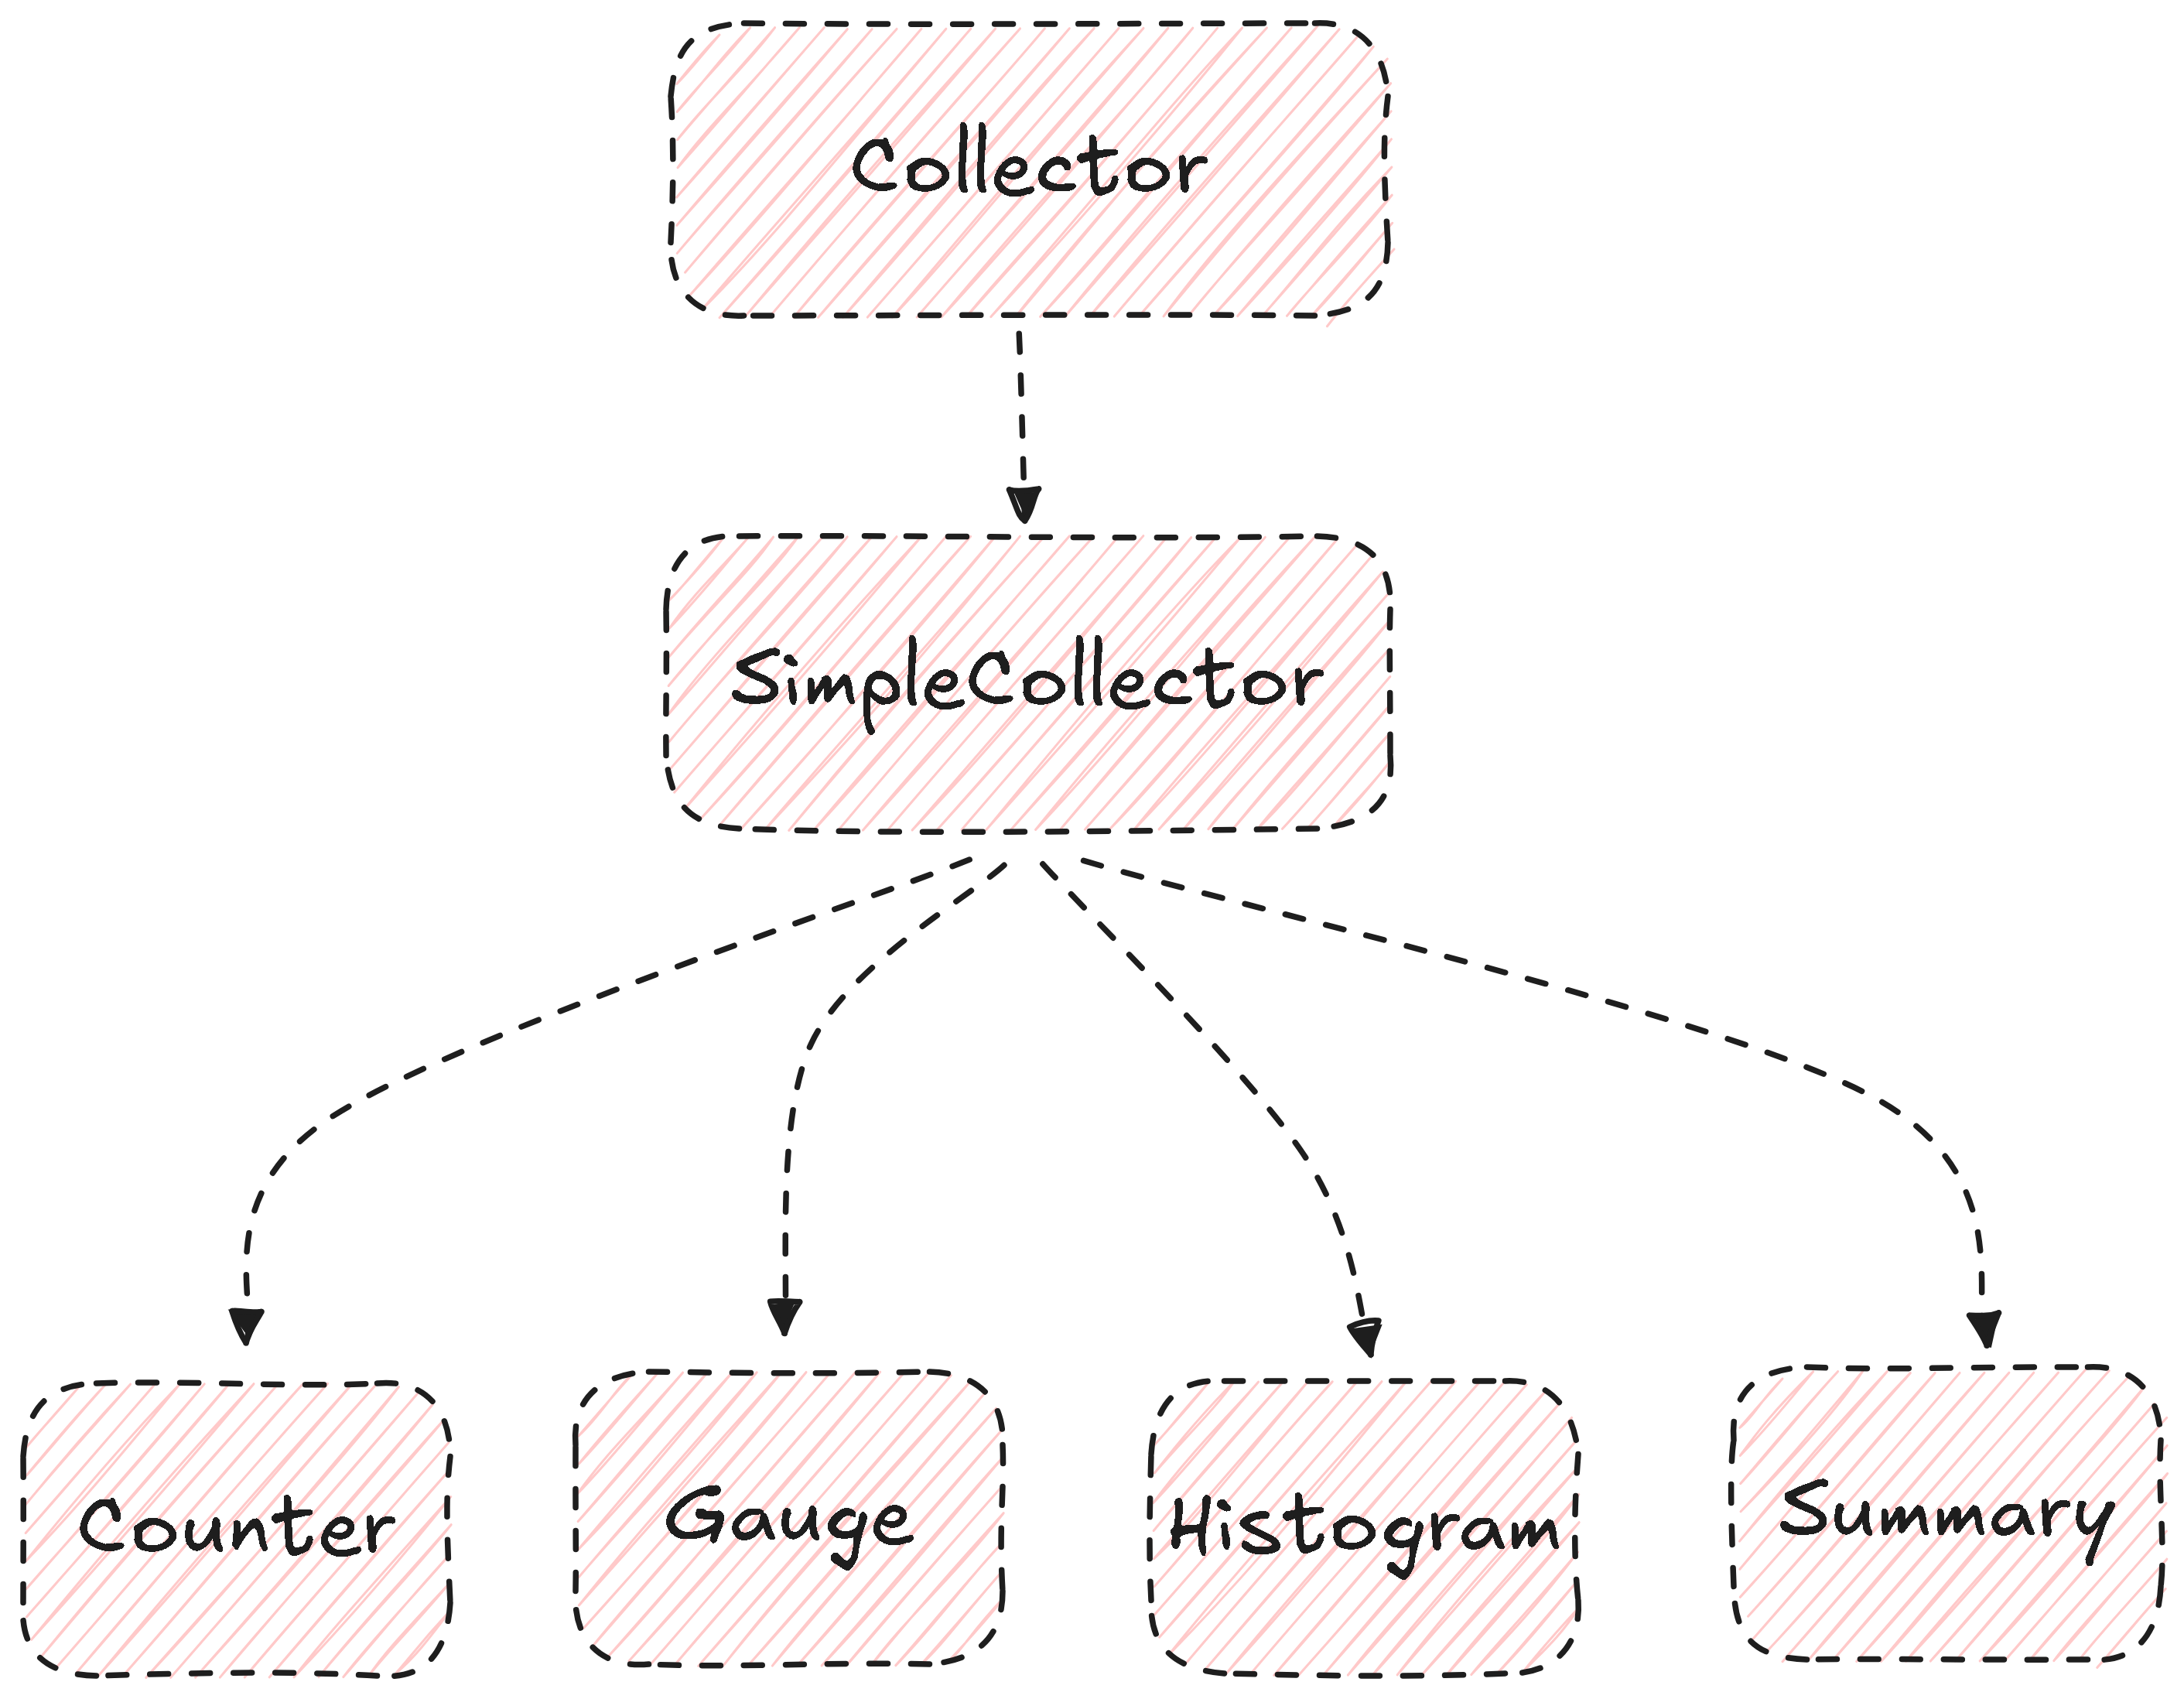
\includegraphics[width=\linewidth, keepaspectratio]{./figures/metric_types}
    \caption{Metric Types}
\end{figure}


\begin{itemize}
    \item \textbf{Counter:} Represents a cumulative metric that only increases, typically used to count discrete events such as requests, errors, or tasks completed.

    \item \textbf{Gauge:} Represents a metric that can increase and decrease arbitrarily, suitable for measuring instantaneous values such as temperature, memory usage, or active sessions.

    \item \textbf{Histogram:} Records observations within configurable buckets to provide a frequency distribution of values, often used for request durations or response sizes.

    \item \textbf{Summary:} Provides streaming quantile estimations, allowing tracking of percentiles (e.g., median, 95th percentile) over a sliding time window.
\end{itemize}

\subsection{Class Hierarchy and Relationships}\label{subsec:class-hierarchy-and-relationships}

The metric types derive from common abstract base classes to promote code reuse and consistent behavior:

All core metric types inherit the \texttt{labels(vararg labelValues: String)} method from their base classes, allowing them to create and retrieve labeled child metrics.
This feature enables dimensionality in metrics by associating key-value label pairs with each observation.

\subsection{Detailed Metric Descriptions}\label{subsec:detailed-metric-descriptions}

\paragraph{Counter}

A \texttt{Counter} is a cumulative metric that can only increase or be reset to zero on restart.
It supports labeled child instances to track counts across different dimensions (e.g., HTTP method and status code).

\begin{itemize}
    \item \texttt{inc()} — Increment the counter by 1.
    \item \texttt{inc(amount: Double)} — Increment the counter by a specified positive amount.
    \item \texttt{get()} — Get the current value of the counter.
\end{itemize}

Example usage:

\begin{lstlisting}
val errors = counter("errors_total") {
    help("Total number of errors")
    labelNames("type")
}

errors.labels("database").inc()
errors.labels("network").inc(2.0)
\end{lstlisting}

\paragraph{Gauge}

A \texttt{Gauge} represents a value that can go up and down, allowing tracking of current states or values that fluctuate.

\begin{itemize}
    \item \texttt{inc()} — Increment the gauge by 1.
    \item \texttt{inc(amount: Double)} — Increment the gauge by a specified amount.
    \item \texttt{dec()} — Decrement the gauge by 1.
    \item \texttt{dec(amount: Double)} — Decrement the gauge by a specified amount.
    \item \texttt{set(value: Double)} — Set the gauge to an explicit value.
    \item \texttt{setToCurrentTime()} — Set the gauge to the current Unix time in seconds.
    \item \texttt{get()} — Get the current value of the gauge.
\end{itemize}

Example usage:

\begin{lstlisting}
val memoryUsage = gauge("memory_usage_bytes") {
    help("Current memory usage in bytes")
}

memoryUsage.set(150_000_000)
memoryUsage.inc(1024)
memoryUsage.dec(512)
\end{lstlisting}

\paragraph{Histogram}

A \texttt{Histogram} samples observations into configurable buckets to represent the frequency distribution of observed values.

\begin{itemize}
    \item \texttt{observe(value: Double)} — Record an observation.
    \item \texttt{clear()} — Reset all recorded data.
\end{itemize}

Histograms automatically count the number of observations and maintain a sum of all observed values to calculate averages.

Example usage:

\begin{lstlisting}
val requestLatency = histogram("http_request_duration_seconds") {
    help("HTTP request latency in seconds")
    buckets(0.1, 0.3, 1.5, 10.0)
}

requestLatency.observe(0.42)
requestLatency.observe(1.2)
\end{lstlisting}

\paragraph{Summary}

A \texttt{Summary} provides streaming quantile estimation, which is useful to calculate percentiles over a sliding time window.

\begin{itemize}
    \item \texttt{observe(value: Double)} — Record a sample observation.
    \item \texttt{clear()} — Reset all data.
\end{itemize}

Example usage:

\begin{lstlisting}
val responseSizes = summary("http_response_size_bytes") {
    help("HTTP response sizes in bytes")
}

responseSizes.observe(512)
responseSizes.observe(1024)
\end{lstlisting}

This metric model provides a consistent and extensible foundation for instrumenting Kotlin applications in a way that aligns with Prometheus best practices.
By leveraging labeled child instances via the inherited \texttt{labels()} method and exposing idiomatic APIs for incrementing, setting, or observing values, the library enables rich and precise metric collection.

\section{DSL and Usability}\label{sec:dsl-and-usability}

To provide an idiomatic and fluent \ac{API} for defining metrics, the library leverages Kotlin’s \ac{DSL} capabilities
combined with builder classes.
While the internal implementation uses builder classes such as \texttt{CounterBuilder} and \texttt{GaugeBuilder} to
encapsulate metric configuration, the user-facing \ac{API} exposes concise \ac{DSL}-style functions that hide the
builder pattern behind expressive Kotlin lambda syntax.

For instance, the \texttt{counter} function allows users to define and register a counter metric in a clear and declarative way:

\begin{figure}[h]
    \begin{lstlisting}
val requests = counter("http_requests_total") {
    help("Total HTTP requests")
    labelNames("method", "status")
    includeCreatedSeries(true)
}
    \end{lstlisting}
    \caption{Counter definition - Prometheus Kotlin library}
\end{figure}

This approach provides several benefits:

\begin{itemize}
    \item \textbf{Simplicity}: Users do not interact directly with builder classes, reducing boilerplate and lowering the barrier to entry.
    \item \textbf{Expressiveness}: The Kotlin lambda with receiver enables a readable, structured way to configure metrics.
    \item \textbf{Flexibility through Defaults}: Configuration fields have sensible defaults, allowing users to specify only the parameters they care about.
    \item \textbf{Optionality}: Most configuration steps are optional, and Kotlin’s support for default and named
    arguments makes the \ac{API} easy to use without requiring verbose setup.
\end{itemize}

In contrast, defining metrics in the Prometheus Java library typically requires more verbose, imperative code that
directly manipulates
builders or configuration objects.
For example, a counter metric might be defined as:


\begin{figure}[h]
    \begin{lstlisting}
Counter.Builder builder = Counter.build()
    .name("http_requests_total")
    .help("Total number of HTTP requests")
    .labelNames("method", "status").register();
    \end{lstlisting}
    \caption{Counter definition - Prometheus Java library}
\end{figure}

This comparison highlights how Kotlin’s language features enable a more elegant and developer-friendly \ac{API}
surface, promoting better usability and reducing common errors.

Similarly, other metric types such as gauges are created using analogous \ac{DSL} functions:

\begin{figure}[h]
    \begin{lstlisting}
val memoryUsage = gauge("memory_usage_bytes") {
    help("Current memory usage in bytes")
    unit("bytes")
    clock(customClock)
}
    \end{lstlisting}
    \caption{Gauge definition - Prometheus Kotlin library}
\end{figure}

Overall, this layered design—with internal builder classes and external \ac{DSL} functions—provides a clear separation
of concerns between metric construction and user interaction, enhancing modularity and maintainability while embracing Kotlin idioms for a modern instrumentation library.


\section{Collector Registry}\label{sec:collector-registry}

The \texttt{CollectorRegistry} class is the central component responsible for managing all metric collectors in the system.
It keeps track of every registered metric and enables the collection of their current state when an exposition is triggered.

This follows the standard model proposed by Prometheus, where collectors (such as counters, histograms, etc.) are registered into a shared registry and later scraped together.

\begin{itemize}
    \item Metrics are explicitly registered using \texttt{CollectorRegistry.register()}.
    \item A global singleton \texttt{defaultRegistry} is provided for convenience in most applications.
    \item The method \texttt{collect()} retrieves a snapshot of all current samples from the registered collectors.
\end{itemize}

The registry is designed to be thread-safe and coroutine-friendly, ensuring safe access from concurrent environments.
Its most common usage is as a backend for metric exposition, such as via \texttt{PrometheusExporter}.

\begin{figure}[h]
    \begin{lstlisting}
val registry = CollectorRegistry.defaultRegistry
registry.register(myCounter)
val samples = registry.collect()
    \end{lstlisting}
    \caption{Collector registration and sample collection}
\end{figure}

Although applications typically rely on the singleton \texttt{defaultRegistry}, custom registries can be created as needed. This is useful for testing, modular system design, or scenarios requiring metric isolation (e.g., multi-tenant services).

\begin{figure}[h]
    \begin{lstlisting}
val myCounter = counter("example_counter") {
    help("An example metric")
}
CollectorRegistry.defaultRegistry.register(myCounter)
    \end{lstlisting}
    \caption{Using the default registry for registration}
\end{figure}


\section{Exposition}\label{sec:exposition}

The exposition component of the library is responsible for converting the collected metrics into the Prometheus 0.0.4 text exposition format, which can be scraped by Prometheus via HTTP. This conversion is handled by the \texttt{PrometheusTextFormat} class and exposed to users via the \texttt{PrometheusExporter}.

\subsection{Text Format Overview}\label{subsec:text-format-overview}

Prometheus expects metrics to be exported as plaintext in a specific structure.
A typical metric exposition includes:

\begin{itemize}
    \item A \texttt{\# TYPE} line specifying the metric type (e.g., counter, gauge).
    \item An optional \texttt{\# UNIT} line.
    \item A \texttt{\# HELP} line describing the metric.
    \item One or more data lines containing the metric name, labels, value, and optionally a timestamp.
\end{itemize}

\begin{figure}[h]
    \begin{lstlisting}
# TYPE http_requests_total counter
# UNIT http_requests_total requests
# HELP http_requests_total Total number of HTTP requests received
http_requests_total{method="GET",status="200"} 1243
    \end{lstlisting}
    \caption{Example metric exposition output}
\end{figure}

\subsection{PrometheusTextFormat}\label{subsec:prometheustextformat}

The \texttt{PrometheusTextFormat} class provides the functionality to encode a list of \texttt{Collector} instances into a single \texttt{String} in the exposition format.
Its main public method is:

\begin{itemize}
    \item \texttt{fun writeMetrics(collectors: List<Collector>, withTimestamp: Boolean = false): String}
\end{itemize}

This method appends, for each collector:

\begin{enumerate}
    \item The metadata lines (\texttt{\# TYPE}, \texttt{\# UNIT}, \texttt{\# HELP}).
    \item The metric sample lines, each representing one time series with optional labels.
    \item If \texttt{withTimestamp} is true, the internal timestamp (in milliseconds since epoch) of each sample is included.
\end{enumerate}

Internally, it uses helper functions:

\begin{itemize}
    \item \texttt{writeMetricMetadata(collector)}: formats and appends the metadata.
    \item \texttt{writeMetricData(collector, withTimestamp)}: serializes all samples of a collector, including label formatting and optional timestamps.
\end{itemize}

Each sample is written as:

\begin{figure}[h]
    \begin{lstlisting}
metric_name{label1="value1",label2="value2"} 123.456 [timestamp]
    \end{lstlisting}
    \caption{Metric sample format}
\end{figure}

Labels are quoted and escaped if needed, and empty label sets are still enclosed in braces (i.e., \texttt{\{\}}).

\subsection{PrometheusExporter}\label{subsec:prometheusexporter}

The \texttt{PrometheusExporter} class serves as the public entry point for metric exposition.
It wraps a \texttt{CollectorRegistry} (defaulting to the global registry) and uses \texttt{PrometheusTextFormat} to serialize its contents.

Its main function:

\begin{itemize}
    \item \texttt{suspend fun scrape(withTimestamp: Boolean = false): String}
\end{itemize}

This suspendable method collects all registered collectors, serializes them via \texttt{writeMetrics()}, and returns the resulting string.
This makes it easy to integrate into coroutine-based HTTP frameworks.

\subsection{Timestamp Support}\label{subsec:timestamp-support}

By default, the exposition omits timestamps to align with Prometheus's preference for assigning scrape time itself.
However, the library tracks timestamps internally for each sample, and the user can enable them explicitly.

This allows applications that require precise client-side timing to expose that data without altering the core logic.

\subsection{Summary}\label{subsec:summary}

The exposition layer provides a clean and extensible mechanism for emitting Prometheus-compatible metrics.
The responsibilities are well-separated:

\begin{itemize}
    \item \texttt{PrometheusTextFormat} focuses on format correctness.
    \item \texttt{PrometheusExporter} simplifies access for application developers.
\end{itemize}

This modular approach ensures that the exposition logic can be reused across different backends and integrated into various HTTP frameworks without duplicating formatting logic.


\section{Benchmarks}

To validate the performance and runtime characteristics of our Kotlin-native Prometheus library, we conducted comparative benchmarks against the official Java Prometheus client. These benchmarks were designed to simulate real-world usage patterns involving high-throughput counter operations, as these are among the most common metrics in production systems.

To simulate asynchronous environments, both clients used a shared \texttt{Channel<Unit>} that dispatches increment signals to a coroutine-based background consumer. This setup closely mirrors usage in high-concurrency environments like HTTP servers or job schedulers.

\subsection*{Benchmark Configuration}
\begin{itemize}
    \item \textbf{Scope}: \texttt{Thread} (isolated state per thread)
    \item \textbf{Benchmark Mode}: \texttt{Throughput}
    \item \textbf{Time Unit}: \texttt{Milliseconds}
    \item \textbf{Channel Buffer}: Size 1024 with \texttt{BufferOverflow.DROP\_OLDEST}
\end{itemize}

\subsection*{Client Implementations}

\textbf{Java Client}: Used the official Prometheus Java library (\texttt{io.prometheus.client.Counter}). Metrics were created and registered globally with a background coroutine processing increment requests.

\textbf{Kotlin Client}: Used our own DSL-based Kotlin implementation (\texttt{io.github.rxfa.prometheus.core.Counter}). The setup mirrors the Java version, including coroutine usage and buffering strategy.

\subsection*{Results Overview}

While exact figures vary depending on runtime conditions, our benchmarks consistently show that:
\begin{itemize}
    \item The Kotlin client offers comparable throughput for each operation, with minimal performance overhead despite its idiomatic and coroutine-centric architecture.
    \item In latency-sensitive paths, the Kotlin client maintains competitive performance by minimizing locking and leveraging Kotlin’s structured concurrency and non-blocking primitives.
\end{itemize}

\subsection*{Takeaways}

The results demonstrate that a fully idiomatic Kotlin Prometheus client can achieve parity with the mature Java implementation in common operational scenarios, while offering a significantly more expressive and safe API surface for Kotlin developers.

This validates our architectural decisions around coroutine integration, label-safe design, and type-safe builders, and provides confidence that our library is suitable for production monitoring workloads in modern Kotlin services.
